\documentclass[12pt,a4paper]{report}
\usepackage[utf8]{vietnam}
\usepackage[utf8]{inputenc}
\usepackage{tabto}
\usepackage{amsmath}
\usepackage{amsfonts}
\usepackage{tikz}
\usepackage{amssymb}
\usepackage{graphicx}
\usepackage[left=2cm,right=2cm,top=2cm,bottom=2cm]{geometry}
\usepackage{graphicx}
\graphicspath{ {./images/} }

\author{Trần Đức Mạnh}
\title{Deep Learning}
\begin{document}
\tableofcontents

\chapter{Introduction to Machine Learning Strategy}
	\section{Why Machine Learing Strategy}
		\begin{itemize}
			\item Đặt vấn đề: Khi xây dựng một Model, để cải thiện hiệu quả của Model đó, bạn đề đặt ra \textbf{rất nhiều} ý tưởng
			\item Nhưng: bạn lại không biết ý tưởng nào giúp cải thiện chất lượng Model, nên bạn chọn một hướng đi như kiểu thu thập thêm dữ liệu mà cuối cùng thì sau 1 
			khoảng thời gian dài bạn có nhiều dữ liệu hơn, nhưng chất lượng Model thì không.
			\item Và đó là lý do mà \textbf{bạn cần có một chiến lược cụ thể}.
		\end{itemize}
	\section{Orthogonalization}
		\begin{itemize}
			\item Ý tưởng: biết phải \textbf{làm gì} để đạt được \textbf{mục 	
			đích gì}
			\item Ví dụ 1: nút để vặn trên TV (TV cổ lắm mới có nút vặn để 
			điều chỉnh).\\ Mỗi một nút vặn sẽ dùng để điều chỉnh một yếu tố 
			duy nhất như là độ rộng của màn hình hay chiều dài của màn hình, 
			hay là độ sáng.
			\item Ví dụ 2: Trong xe ô tô phải có vô lăng để điều chỉnh hướng 
			đi của xe, và chân ga để tăng tốc hay phanh để giảm tốc.\\
			Giả sử nếu tất cả yếu tố, hướng đi của xe, tăng tốc, giảm tốc đều 
			phụ thuộc vào vô lăng không thôi thì sẽ rất khó để điều khiển xe.
			\item Khi train Model cũng giống như thế, bạn nhìn vào vấn đề mà 
			bạn đang đối mặt với ví dụ như Model của bạn hoạt động không tốt 
			trên Test Set thì lúc đó bạn sẽ "vặn cái nút nào" để giải quyết 
			vấn đề.\\ Và mỗi cái nút mà bạn sắp vặn, nó nên chỉ ảnh hưởng đến 
			một yếu tố của Model (vì có một số "nút" - thuật toán - ảnh hưởng 
			đến nhiều hơn một yếu tố của Model.
		\end{itemize}
\chapter{Setting Up your Goal}
	\section{Single Number Evaluation Metric}
		\begin{itemize}
			\item Tiếng Việt: đơn chỉ số đánh giá
			\item Quá trình xây dựng Model: \\ 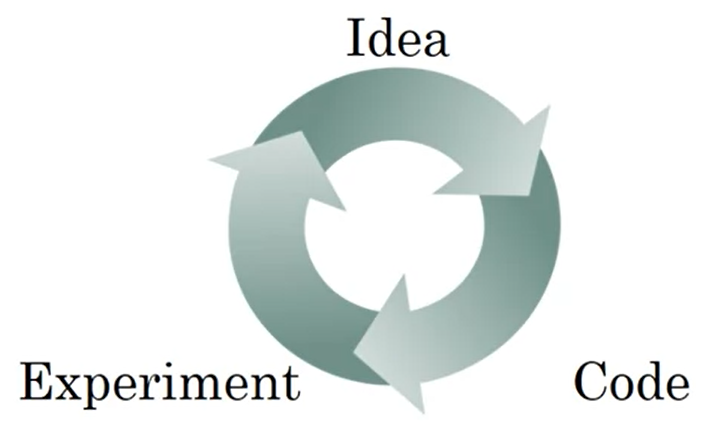
\includegraphics[scale=0.5]{1}
			\item Precision \& Recall
				\begin{itemize}
					\item Ví dụ trong nhận diện ảnh Mèo:
						\begin{itemize}
							\item Precision là "Trong số các ví dụ được nhận 
							diện là Mèo, thì có bao nhiêu \% ví dụ đó thật sự 
							là Méo"
							\item Recall là "Có bao nhiêu ví dụ Méo được nhận 
							diện đúng"
						\end{itemize}
					\item Ví dụ: \\
						\begin{tabular}{ | c | c c | }
							\hline
							Classifier & Precision & Recall \\ 
							\hline
							A & 95\% & 90\% \\  
						 	B & 98\% & 85\% \\
						 	\hline
						\end{tabular}
					\item Vấn đề đặt ra: Nếu dùng 2 thông số Precision và 
					Recall thì sẽ rất khó để đánh giá thuật Classifier nào là 
					tốt hơn (vì Classifier A có Recall cao hơn, còn B thì 
					Precision cao hơn).
					\item Để giải quyết vấn đề trên, ta có thể dùng 1 thông 
					số mới - "Trung bình" của 2 thông số trên - để đánh giá\\
						\begin{tabular}{ | c | c c c | }
							\hline
							Classifier & Precision & Recall & F1 Score \\ 
							\hline
							A & 95\% & 90\% & 92.4\% \\  
						 	B & 98\% & 85\% & 91.0\% \\
						 	\hline
						\end{tabular}
						\begin{itemize}
							\item F1 Score = "Trung bình" của Precision (P) 
							và Recall (R)
							\item $ \text{F1 Score} = \frac{2}{\frac{1}{P} + 
							\frac{1}{R}} $ (được gọi là \textbf{Harmonic 
							Mean})
						\end{itemize}
					\item Bây giờ dễ thấy rằng Classifier nào tốt hơn
				\end{itemize}
			\item Tóm lại: Bằng cách xác định từ đầu, trước khi xây dựng 
			Model, quyết định những đơn thông số để đánh giá thuật toán sẽ 
			giúp việc quyết định Model nào là tốt hơn Model nhanh hơn, dễ hơn.
		\end{itemize}
	\section{Satisficing and Optimizing Metric}
		\begin{itemize}
			\item Ví dụ 1: Cat Classification
				\begin{itemize}
					\item Bảng: \\
						\begin{tabular}{|c | c c |}
							\hline
							Classifier & Accuracy & Running Time \\
							\hline
							A & 90\% & 80ms \\
							B & 92\% & 95ms \\
							C & 95\% & 1500ms \\
							\hline
						\end{tabular}
					\item \textbf{Cách không hiệu quả:} $ \text{Cost} = 
					\text{Accuracy} - 0.5 \times \text{Running Time} $
					\item \textbf{Cách hiệu quả: } Maximize Accuracy subject 
					to Running Time $ \leq $ 100ms
						\begin{itemize}
							\item Maximize Accuracy: tối ưu thông số Accuracy
							$\xrightarrow{}$ Accuracy: \textbf{Optimizing\\ 
							Metric}
							\item Subject to Running Time $ \leq $ 100ms: tuy 
							thuộc vào thông số Running Time nếu $ \leq $ 
							100ms\\
							Running time được gọi là \textbf{Satisficing 
							Metric} vì tao chỉ quan tâm đến nó trong một 
							ngưỡng (threshold) nhất định, nếu lớn hơn thì
							bỏ qua
						\end{itemize}
				\end{itemize}
			\item Ví dụ 2: Wakewords/Trigger words
				\begin{itemize}
					\item Trigger words: Alexa, Ok Google, Hey Siri, \ldots 
					dùng trong trợ lý ảo
					\item Ở bài toán này tao muốn: \textbf{Maximize 	
					Accuray} \textit{(Độ chính xác của việc khi nói trigger 
					word thì trợ lý ảo khởi động)} \textbf{subject to $\leq$ 
					1 false postive every 24 hours} \textit{(xác suất thức 
					dậy của trợ lý ảo dù không nói gì trong 24 giờ)}
				\end{itemize}
		\end{itemize}
	\section{Train/Dev/Test Distributions}
		\begin{itemize}
			\item Khi chia Data thành Dev set và Test set thì phải \textbf{phân 
			bố đều} trên cả 2
			\item Ví dụ: bạn có Data của 8 khu vực: US, UK, Europe, South 
			America, India, China, Australia, Vietnam\\
			Và bạn chia Dev set là 4 khu vực bất kì, Test set là 4 khu vực còn 
			lại.\\
			Thì như thế là không tốt, vì Dev và Test có phân bố khác nhau.\\
			Nó giống như kiểu, bạn luyện tập để bắn vào 1 cái bia vậy, nhưng 
			lúc đi thi đấu thì cái bia ý lại được đặt ở vị trí khác, xa hơn, 
			chéo hơn khiến bạn không bắn được.\\
			Việc phân bố Dev và Test set không đều cũng giống như thế.
			\item Guideline: \textbf{Choose a dev set and test set to reflect
			data you expect to get in the future and consider important to do
			well on} (Dev và Test set phải có cùng phân bố (same 
			distribution))
		\end{itemize}
	\section{Size of the Dev and Test Sets}
		\begin{itemize}
			\item Ngày xưa khi không nhiều Data (100 - 10.000 training 
			examples)
			thì người ta thường hay chia thành 70\% Train, 30\% Dev hoặc 60\% 
			Train, 20\% Dev, 20\% Test
			\item Nhưng ngày nay, với số lượng Data khủng lổ (1.000.000 
			training examples) thì việc chia như thế kia không còn hợp lý nữa
			\item Với số lượng Data lớn thì chia \textbf{98\% Train, 1\% Dev, 
			1\% Test} sẽ hợp lý hơn
			\item Với Dev và Test set thì khoảng 10.000 training examples là 
			ổn
			\item Có thể không có Test set, nhưng Train và Dev là phải có, 
			điều này không được khuyến khích\\ (Nếu ai đó nói chỉ có Train và 
			Test thì Test của họ là Dev)
		\end{itemize}
	\section{When to Change Dev/Test Sets and Metrics?}
		\begin{itemize}
			\item Ví dụ 1: bạn chọn Metric cho 1 model Cat classification như 
			sau:\\
			\tabto{0.5cm} Metric: Classification Error
			\tabto{0.5cm} Classifier A: 3\% Error
			\tabto{0.5cm} Classifier B: 5\% Error
				\begin{itemize}
					\item Nhìn vào dễ thấy Classifier A làm việc tốt hơn
					\item Nhưng mà Classifier A lại gắn mác cho pornographic 
					là Cat, trong khi Classifier B thì không
					\item Tức là ở góc nhìn của Người dùng, thì họ sẽ thấy 
					Classifier B hoạt động tốt hơn
				\end{itemize}
			\item Ví dụ 2: Vẫn như ví dụ 1, nhưng mà Metric + Dev/Test set của 
			bạn lại được chạy trên những hình ảnh Mèo chất lượng cao. Nhưng 
			người dùng lại sử dụng toàn những hình ảnh mờ, lạ, chất lượng xấu.
			\\ Lúc này, Classifier B lại hoạt động tốt hơn A trên những hình 
			ảnh xấu đó.
			\item Những ví dụ trên là lúc mà bạn phải đổi hướng, chọn Metric 
			+ Dev/Set mới
		\end{itemize}
\chapter{Comparing to Human-level Performance}
	\section{Why Human-level Performance?}
		\begin{itemize}
			\item Nhận xét về đồ thị sau:\\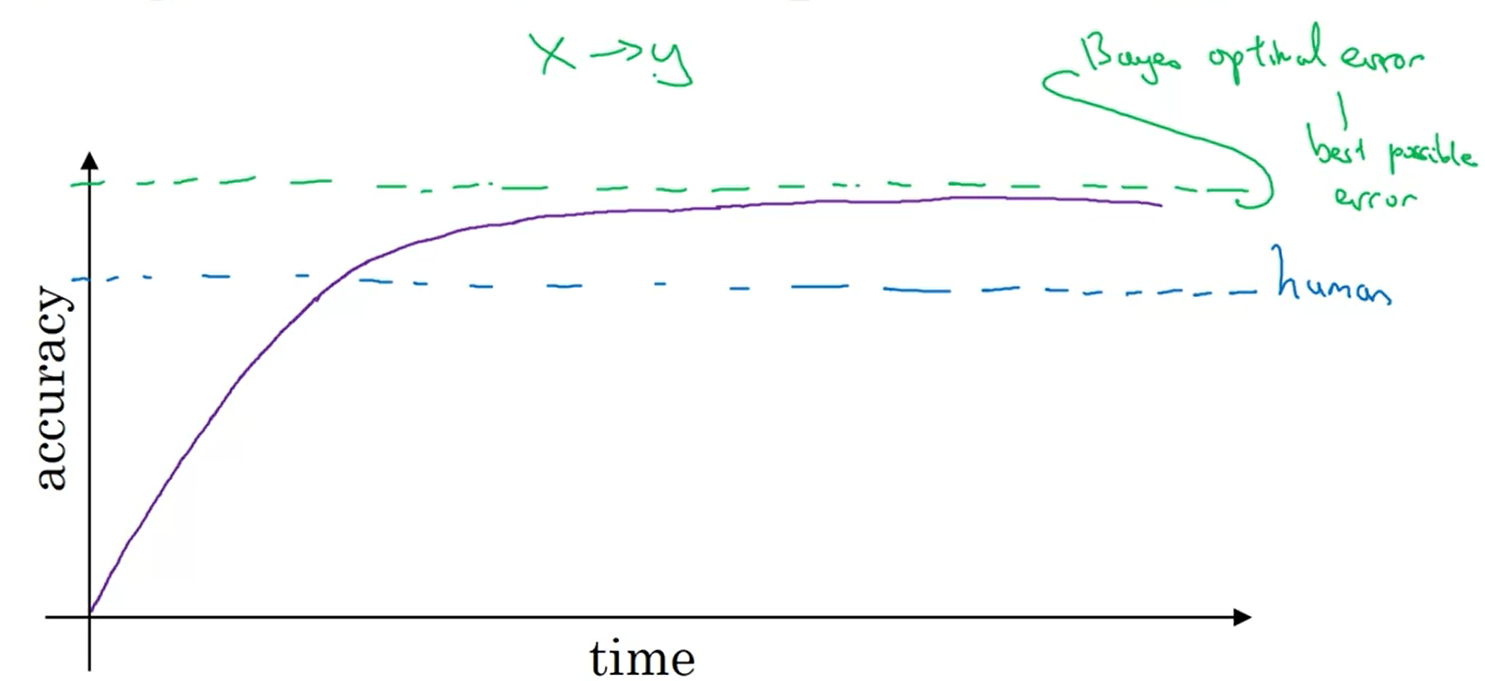
\includegraphics[scale=0.35]{3}
				\begin{itemize}
					\item Đây là đồ thị thể hiện độ chính xác của thuật toán theo thời gian.
					\item Ta có thể thấy độ chính xác của thuật toán chạm đến độ chính xác của con người trong khoảng thời gian rất ngắn.
					\item Thuật toán có thể vượt qua độ chính xác của con người, nhưng rồi sẽ chạm đến một cái giới hạn gọi là \textbf{Bayes Optimal Error}.
					\item Khoảng cách giữa Bayes Error (cách gọi tắt của Bayes Optimal Error) với độ chính xác của con người là rất ngắn vì con người khá giỏi trong việc nhận diện các vấn đề của AI nói chung.
				\end{itemize}
			\item Lý do so sánh độ chính xác của thuật toán với con người: chừng nào độ chính xác của thuật toán vẫn chưa chạm được đến độ chính xác của con người, thì tức là ta vẫn có thể cải thiện thuật toán qua những cách sau:
				\begin{itemize}
					\item Để con người gán label cho data
					\item Tìm hiểu lỗi bằng cách phân tích thủ công
					\item Phân tích tốt hơn về Bias/Variance
				\end{itemize}
		\end{itemize}
	\section{Avoidable Bias}
		\begin{itemize}
			\item Cho bảng sau:\\
				\begin{tabular}{l|c|c}
				Human ($\approx$ Bayes)&1\%&7.5\%\\
				\hline
				Training Error&8\%&8\%\\
				Dev Error&10\%&10\%\\				
				\end{tabular}
			\item Trong ví dụ này, giả sử như là nhận diện ảnh, thì chúng ta có thể chọn Human-level Error làm Bayes Error vì con người có khả năng nhận diện ảnh rất tốt. Đối với Computer Vision (CV) thì cách chọn Bayes Error này khá hợp lý.
			\item $\text{Avoidable Bias} = \text{Training Error} - \text{Humun-level Error}$
			\item $\text{Variance} = \text{Dev Error} - \text{Training Error}$
			\item Ở cột 1: Vì Avoidable Bias (7\%) cao hơn Variance (2\%) nên sẽ tốt hơn nếu bạn tập trung vào việc làm giảm Bias trước
			\item Ở cột 2: Vì Avoidable Bias (0.5\%) nhỏ hơn Variance (2\%) nên sẽ tốt hơn nếu bạn tập trung vào việc làm giảm Variance trước
		\end{itemize}
	\section{Understanding Human-level Performance}
		\begin{itemize}
			\item Thế nào là Human-level Performance?
				\begin{itemize}
					\item Trong vấn đề chuẩn đoán bệnh qua ảnh:
						\begin{itemize}
							\item 1 người thường: 3\% Error
							\item 1 bác sĩ: 1\% error
							\item 1 bác sĩ nhiều kinh nghiệm: 0.7\%
							\item 1 nhóm bác sĩ nhiều kinh nghiệm: 0.5\%
						\end{itemize}
					\item Vậy thì đâu mới là giá trị hợp lý cho Human-level Performance?
				\end{itemize}
			\item Ví dụ:\\
				\begin{tabular}{l|c|c|c}
					Human ($\approx$ Bayes)&0.5-1\%&0.5-1\%&0.5\%\\
					\hline
					Train Error&5\%&1\%&0.7\%\\
					Dev Error&6\%&5\%&0.8\%\\
					&Bias&Variance&\\
				\end{tabular}
				\begin{itemize}
					\item Ở cột 1 ta chọn giá trị cho Human-level Error trong khoảng từ 0.5-1\% đều có thể thấy rằng Avoidable Bias lớn hơn Variance, nên ở trường hợp này thì ta nên tập trung vào xử lý Bias
					\item Ở cột 2 thì rõ ràng thấy được Variance lớn hơn Avoidable Bias nên tao tập trung vào xử lý Variance
					\item Còn ở cột 3, thì nếu như ta chọn Human-level Error là 0.7\% thay cho 0.5\% trong ảnh thì sẽ thấy Variance lớn hơn Avoidable Bias, nhưng với 0.5\% thì ta thấy điều ngược lại\\$\rightarrow$ Tức là khi mà thuật toán đã trở nên tốt hơn, gần đạt tới Human-level Performance thì việc chọn Human-level Error nào sẽ ảnh hưởng nhiều hơn khi mà thuật toán còn làm việc chưa tốt
				\end{itemize}
			\item Tóm lại việc chọn Human-level Error nào sẽ có ảnh hưởng đến việc quyết định xử lý Bias hay Variance
		\end{itemize}
	\section{Surpassing Human-level Performance}
		\begin{itemize}
			\item 1 vấn đề nảy sinh khi thuật toán vượt qua Human-level Performance là lúc đó bạn sẽ không thể biết được là nên chọn giá trị Bayes Error như thế nào để tiếp tục khiến thuật toán của bạn tốt hơn.\\$\rightarrow$ Đó là lý do tại sao mà sau khi vượt Human-level Performance, các thuật toán rất khó để phát triển hơn nữa.
			\item Đến bây giờ đã xuất hiện rất nhiều những lĩnh vực, mà AI vượt qua con người, như trong nhận diện ảnh, hay nhận diện giọng nói.
		\end{itemize}
	\section{Improving your Model Performance}
		\begin{itemize}
			\item Avoidable Bias:	
				\begin{itemize}
					\item Train bigger model
					\item Train longer/better optimization algorithms
					\item NN architecture/hyperparameters search (như CNN, RNN)					
				\end{itemize}
			\item Variance:
				\begin{itemize}
					\item More data
					\item Regularization (L2, dropout, ...)
					\item NN architecture/hyperparameters search (như CNN, RNN)					
				\end{itemize}
		\end{itemize}
\chapter{Error Analysis}
	\section{Carrying Out Error Analysis}
		\begin{itemize}
			\item Các bước phân tích lỗi:
				\begin{enumerate}
					\item Tìm 1 tập các ví dụ bị gắn nhầm Label trong Dev set hoặc Test set
					\item Tìm các ví dụ \textbf{false positives} và \textbf{false negatives} trong đó
					\item Đếm số lượng sai trong các mục lỗi khác nhau
					\item Trong quá trình bạn có thể gặp mục lỗi mới
					\item Từ đó quyết định xử lý lỗi nào trước hoặc đi theo 1 hướng mới
				\end{enumerate}
			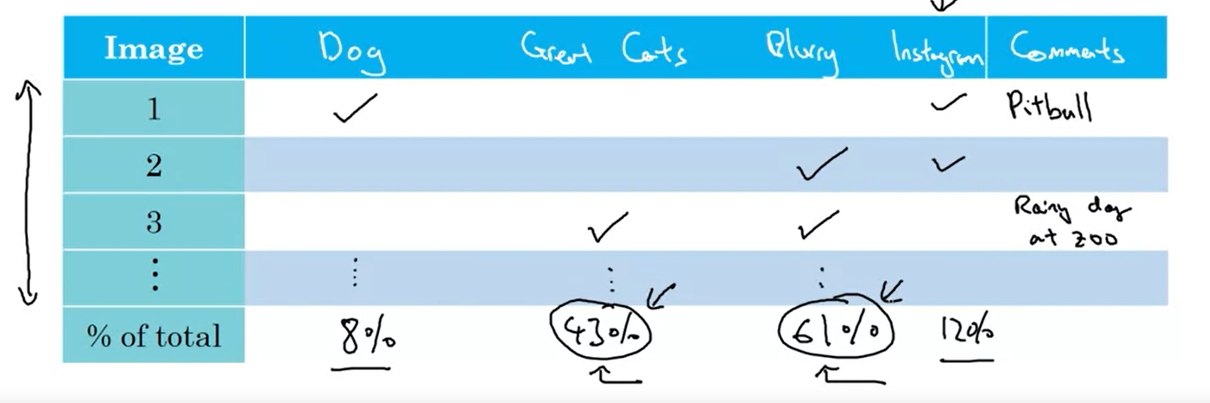
\includegraphics[scale=0.4]{4}
		\end{itemize}
	\section{Cleaning Up Incorrectly Labeled Data}
		\begin{itemize}
			\item Câu hỏi đầu tiên được đặt ra là \textbf{Nó có đáng không?}\\Vì có thể việc gán sai nhãn cho một vài ví dụ một cách \textbf{ngẫu nhiên} không làm ảnh hưởng quá nhiều đến tổng thể\\Nếu là lỗi một cách \textbf{hệ thống} thì chắc chắn cần phải xem xét
			\item Bằng cách thêm 1 cột \textbf{"Incorrectly labeled"} vào bảng trên có thể giúp bạn quyết định là việc chỉnh lại nhãn cho đúng có đáng hay không
			\item Một số lưu ý:
				\begin{itemize}
					\item Áp dụng cùng 1 quá trình lên cả Dev và Test set để đảm bảo cả 2 có cùng phân bố (distribution)
					\item Xem xét cả những ví dụ đúng cùng với ví dụ sai
					\item Tran và Dev/Set có thể trở nên hơi khác về phân bố (distribution)
				\end{itemize}
		\end{itemize}
	\section{Build your First System Quickly, then Iterate}
		\begin{itemize}
			\item Thay vì xây dựng 1 hệ thống phức tạp từ đầu, hãy xây dựng 1 hệ thống đơn giản nhanh chóng rồi từ đó, dựa vào phân tích Bias/Variance và Error để quyết định hướng đi sẽ nhanh hơn trong việc tạo ra 1 hệ thống hoạt động
		\end{itemize}
\chapter{Mismatched Traing and Dev/Test Set}
	\section{Training and Testing on Different Distributions}
		\begin{itemize}
			\item Nếu bạn 500.000 data kiểu A và 20.000 data kiểu B mà bạn lại muốn hệ thống của mình hoạt động tốt trên B thì bạn nên chia data kiểu B thành 10.000, 5.000, 5.000 rồi chia Train/Dev/Test như sau:\\
			\begin{tabular}{|p{0.6\linewidth}|p{0.1\linewidth}|p{0.1\linewidth}|}
				\hline
				500.000 A + 10.000 B & 5.000 B & 5.000 B\\
				\hline
			\end{tabular}
			\item Không nên trộn hết vào rồi random chúng
		\end{itemize}
	\section{Bias and Variance with Mismatched Data Distributions}

	\section{Addressing Data Mismatch}
\chapter{Learning from Multiple Tasks}
	\section{Transfer Learning}
	\section{Multi-task Learing}
\chapter{End-to-end Deep Learning}
	\section{What is End-to-end Deep Learning?}
	\section{Whether to use End-to-end Deep Learning}
\end{document}
